\section{Particle-Mode Interaction and Optical Depth}
\begin{figure}[!htb]
	\centering
	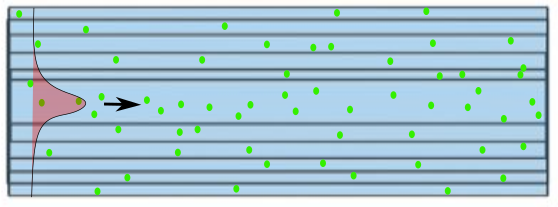
\includegraphics[width=0.5\textwidth]{./Figures/ICG/icgfibermode.png}
	\caption{Diagram of a Gaussian mode traveling through a fully-filled HCPBF with normally suspended nanoparticles.}
	\label{fig:icg_mode}
\end{figure}
Optical depth (OD) is a measurement of the opacity of a system, related to the transmitted intensity by $T = exp(-OD)$. With particles distributed throughout the fiber, the interaction between the beam and particles inside the fiber needs to be taken into account. When considering a single particle interacting with the mode function of a waveguide the strength of the particle interaction will depend on its position within the mode\cite{domokos, mazoni}. The effective mode area of the waveguide is then relevant only in relation to the position of the particle. 
\begin{equation}
	\sigma_M = \frac{\int dxdy|f_k(x, y)|^2}{|f_k(x_p, y_p)|^2}
\end{equation}
where $f_k(x,y)$ is the transverse mode function and $f(x_p,y_p )$ is the position of the particle. In the case of a Gaussian mode function (as would be in a HCPBF), the photon interaction with the particle will be stronger in the center of the mode and weak at the edges. The optical depth (OD) for a single particle the ratio of the scattering cross-section to that of the effective mode-area $OD =\frac{\sigma_0}{\sigma_M}$, so to find the optical depth over the entire ensemble the product of the number density of the sample and optical depth of each emitter is integrated over the volume :
\begin{equation}
	\begin{aligned}
		OD_{fiber} &= \int^{L'}_0 \int^{r'}_0 n(r, z)OD(2\pi r) dr dz 
	\end{aligned}
\end{equation}
where $r'$ and $L'$ represent the radius and length of the ensemble.  When the fibers are fully liquid cladding and core, due to the low interaction and guidance of photons in the PC structure, an approximation is made constricting the mode function strictly to the core. This simplifies the dimensions of the integration to just be the radius and length of the fiber. This assumes that the particulates outside of the core do not have a significant contribution.  If the distribution of molecules is taken to be uniform along the fiber length and radius of the core, then the number density is: 
\begin{equation}
	n(r, z) = \frac{N_{particle}}{V_{fiber}} = \frac{N_{particle}}{\pi r_{core}^2L_{fiber}} 
\end{equation}
The integral will simplify to
\begin{equation}
	\begin{aligned}
		OD_{fiber} &= \int^{L_{fiber}}_0 \int^{r_{core}}_0  n(r_{core}, L_{fiber})\sigma_0 \frac{2}{\pi w_0^2}e^{-\frac{2r^2}{w_0^2}}(2\pi r) dr dz\\
		&= N_{particle}\frac{\sigma_0}{\pi r^2_{core}}\big(1-e^{\frac{-2r_{core}^2}{w_0^2}}\big)
	\label{OD}
	\end{aligned}
\end{equation}